\documentclass[11pt,a4paper]{article}
\usepackage[margin=2.2cm]{geometry}
\usepackage{amsmath,amssymb,bm}
\usepackage{graphicx,float,booktabs,caption,subcaption}
\usepackage{xcolor}
\usepackage{listings}
\usepackage{tikz}
\usetikzlibrary{shapes.geometric,arrows.meta,positioning,calc}
\usepackage[colorlinks=true,linkcolor=blue!50!black,urlcolor=blue!50!black,citecolor=blue!50!black]{hyperref}
\usepackage{fancyhdr}
\pagestyle{fancy}\fancyhf{}\lhead{\small Karthick J (OE23S018), IIT Madras}\rhead{\small\leftmark}\cfoot{\thepage}
\definecolor{codebg}{rgb}{0.97,0.97,0.97}
\lstset{basicstyle=\ttfamily\scriptsize,backgroundcolor=\color{codebg},frame=single,breaklines=true,
 keywordstyle=\color{blue!60!black}\bfseries,commentstyle=\color{green!40!black},stringstyle=\color{red!50!black},
 numbers=left,numberstyle=\tiny\color{gray},showstringspaces=false,tabsize=4,columns=fullflexible,
 literate={²}{{$^2$}}1 {³}{{$^3$}}1 {°}{{$^\circ$}}1 {Δ}{{$\Delta$}}1 {ρ}{{$\rho$}}1 {μ}{{$\mu$}}1 {ω}{{$\omega$}}1 {ψ}{{$\psi$}}1 {α}{{$\alpha$}}1 {ν}{{$\nu$}}1 {τ}{{$\tau$}}1 {–}{{-}}1 {—}{{-}}1 {’}{{'}}1 {“}{{"}}1 {”}{{"}}1 {→}{{$\to$}}1 {≤}{{$\le$}}1 {≥}{{$\ge$}}1 {×}{{$\times$}}1 {±}{{$\pm$}}1 {·}{{$\cdot$}}1 {∂}{{$\partial$}}1 {∇}{{$\nabla$}}1 {γ}{{$\gamma$}}1 {ε}{{$\varepsilon$}}1 {μ}{{$\mu$}}1 {├}{{+}}1 {─}{{-}}1 {│}{{|}}1 {▶}{{>}}1 {▼}{{v}}1 {┌}{{+}}1 {┐}{{+}}1 {└}{{+}}1 {┘}{{+}}1 {┬}{{+}}1 {┴}{{+}}1}
\tikzset{
 startstop/.style={rectangle,rounded corners=6pt,minimum width=3.2cm,minimum height=0.8cm,text centered,draw=black,fill=red!12,font=\small},
 process/.style={rectangle,minimum width=4.6cm,minimum height=0.8cm,text centered,text width=5.6cm,draw=black,fill=blue!8,font=\small},
 decision/.style={diamond,aspect=2.6,text centered,text width=3.2cm,draw=black,fill=green!12,font=\small,inner sep=1pt},
 io/.style={trapezium,trapezium left angle=72,trapezium right angle=108,minimum width=3.6cm,minimum height=0.8cm,text centered,text width=4.6cm,draw=black,fill=orange!15,font=\small},
 arrow/.style={thick,-{Stealth[length=2.5mm]}}}
\setlength{\parskip}{4pt}\setlength{\parindent}{0pt}

\title{\textbf{Two-Dimensional Poisson Equation on the Unit Square}\\[2pt]\large Jacobi, Gauss--Seidel and Successive Under-Relaxation Solvers in C: Accuracy, Convergence and Stopping Criteria\\[2pt]\normalsize Course Project 4 -- OE5450 Numerical Techniques in Ocean Hydrodynamics (Assignment 3, Jan--May 2025)}
\author{Karthick J (OE23S018)\\Department of Ocean Engineering, IIT Madras\\Faculty: Prof.\ K.\ Murali}
\date{Revised report, October 2026}
\begin{document}\maketitle
\begin{abstract}
The Poisson equation $\nabla^2T=Q$ with a two-node source/sink pair is solved on the unit square for two sets of boundary conditions (Dirichlet on all walls; and Dirichlet on three walls with a prescribed flux $\partial T/\partial x=-1$ on the fourth) and three grids ($\Delta=0.1,0.05,0.01$) with point Jacobi, Gauss--Seidel and successive under-relaxation (SUR, $\alpha=0.7$). Review of the submitted C codes found an out-of-bounds write in the Jacobi boundary routine, boundary conditions rotated by $90^\circ$ relative to the problem statement, a floating-point truncation that moved one source to $x=0.44$, per-iteration output of the whole field (up to 0.7~GB per run), and no implementation of Case~2. After correction, all solvers converge to the direct sparse solution of the discrete system, which agrees with the analytical Laplace solution with second-order accuracy ($3.3\times10^{-4}$ interior error at $\Delta=0.01$). The study shows that the absolute increment test $\max|T^{k+1}-T^k|<10^{-4}$ leaves an iteration error of order $\epsilon\rho/(1-\rho)$, i.e.\ $0.10$--$0.21$ on the finest grid, more than half of the solution magnitude in Case~2; a tolerance of $10^{-6}$ reduces it to $10^{-3}$. Iteration counts grow as $N^2=\Delta^{-2}$, as predicted by $\rho_J=\cos\pi\Delta$.
\end{abstract}
\tableofcontents\newpage

\section{Problem definition}
\begin{equation}
\frac{\partial^2T}{\partial x^2}+\frac{\partial^2T}{\partial y^2}=Q(x,y),\qquad 0\le x,y\le1, \label{eq:poisson}
\end{equation}
with nodal sources $Q=+1$ at $(0.45,0.5)$ and $Q=-1$ at $(0.55,0.5)$ (zero elsewhere).
\begin{table}[H]\centering\small
\begin{tabular}{lll}\toprule
& Case 1 & Case 2\\\midrule
$y=0$, $y=1$ & $T=0$ & $T=0$\\
$x=0$ & $T=10$ & $T=0$\\
$x=1$ & $T=10$ & $\partial T/\partial x=-1$\\\bottomrule
\end{tabular}\caption{Boundary conditions (from the problem statement).}\end{table}
Grid spacings $\Delta=\Delta x=\Delta y=0.1,\,0.05,\,0.01$ ($N=1/\Delta=10,20,100$) were to be compared, using Jacobi, Gauss--Seidel and successive under-relaxation iterations with the stopping criterion $\max|T^{k+1}_{ij}-T^k_{ij}|<10^{-4}$.

\subsection{Analytical solution of the source-free problem}
Because $Q$ is non-zero at only two nodes, its effect on $T$ is very small (Section~\ref{sec:source}), and the analytical Laplace solutions provide the accuracy reference:
\begin{align}
\text{Case 1:}\quad T&=\sum_{n\ \mathrm{odd}}\frac{40}{n\pi}\sin(n\pi y)\,\frac{\cosh\!\big(n\pi(x-\tfrac12)\big)}{\cosh(n\pi/2)},\\
\text{Case 2:}\quad T&=-\sum_{n\ \mathrm{odd}}\frac{4}{n^2\pi^2}\sin(n\pi y)\,\frac{\sinh(n\pi x)}{\cosh(n\pi)},
\end{align}
the second following from expanding the boundary flux $-1=\sum b_n\sin n\pi y$, $b_n=-4/(n\pi)$ for odd $n$. Case~1 has temperature discontinuities at the four corners, which limit pointwise accuracy there; errors are therefore measured on $[0.2,0.8]^2$.

\section{Numerical method}
\subsection{Discretisation}
The five-point central approximation of \eqref{eq:poisson} on a uniform mesh is
\begin{equation}
T_{i+1,j}+T_{i-1,j}+T_{i,j+1}+T_{i,j-1}-4T_{i,j}=\Delta^2Q_{i,j},\qquad \tau=\frac{\Delta^2}{12}\big(T_{xxxx}+T_{yyyy}\big)+\mathcal{O}(\Delta^4). \label{eq:5pt}
\end{equation}
The Case~2 flux condition is closed with the second-order one-sided formula
\begin{equation}
\frac{3T_{N,j}-4T_{N-1,j}+T_{N-2,j}}{2\Delta}=-1\quad\Longrightarrow\quad T_{N,j}=\tfrac13\big(4T_{N-1,j}-T_{N-2,j}-2\Delta\big),
\end{equation}
applied after every sweep.

\subsection{Iterative schemes}
Writing \eqref{eq:5pt} as $A\mathbf{T}=\mathbf{b}$, $A=D-L-U$:
\begin{align}
\text{Jacobi:}\quad& T^{k+1}_{ij}=\tfrac14\big(T^k_{i+1,j}+T^k_{i-1,j}+T^k_{i,j+1}+T^k_{i,j-1}-\Delta^2Q_{ij}\big), &\rho_J&=\cos\pi\Delta,\\
\text{Gauss--Seidel:}\quad& T^{k+1}_{ij}=\tfrac14\big(T^{k+1}_{i-1,j}+T^{k}_{i+1,j}+T^{k+1}_{i,j-1}+T^{k}_{i,j+1}-\Delta^2Q_{ij}\big), &\rho_{GS}&=\rho_J^2,\\
\text{SUR:}\quad& T^{k+1}_{ij}=T^k_{ij}+\alpha\big(\tilde T^{GS}_{ij}-T^k_{ij}\big),\ \alpha=0.7, &\rho_{SUR}&\approx1-\alpha(1-\rho_{GS}).
\end{align}
For $\Delta=0.1,\,0.05,\,0.01$: $\rho_J=0.9511,\,0.9877,\,0.99951$ and $\rho_{GS}=0.9045,\,0.9755,\,0.99901$. The number of iterations to reduce the error by a fixed factor is $\propto1/(1-\rho)\approx2/(\pi^2\Delta^2)$ for Jacobi, i.e.\ it grows as $N^2$. Gauss--Seidel needs half as many, and under-relaxation ($\alpha<1$) makes SUR \emph{slower} than Gauss--Seidel by about $1/\alpha$. Under-relaxation is useful for non-linear or stiff problems, not for the linear Poisson equation, for which over-relaxation ($\omega\approx2/(1+\sin\pi\Delta)$) is optimal.

\subsection{Stopping criterion and iteration error}
For a linear stationary iteration with spectral radius $\rho$, the error $e^k=T^k-T$ and the increment $\delta^k=T^{k+1}-T^k$ are related asymptotically by
\begin{equation}
\|e^{k+1}\|\approx\frac{\rho}{1-\rho}\,\|\delta^k\| .\label{eq:err}
\end{equation}
With $\|\delta\|<\epsilon=10^{-4}$ and $\Delta=0.01$ this gives $e\approx0.20$ for Jacobi and $0.10$ for Gauss--Seidel: the increment test is far looser than it appears on fine grids. This is quantified in Section~\ref{sec:conv}.

\subsection{Algorithm}
\begin{figure}[H]\centering
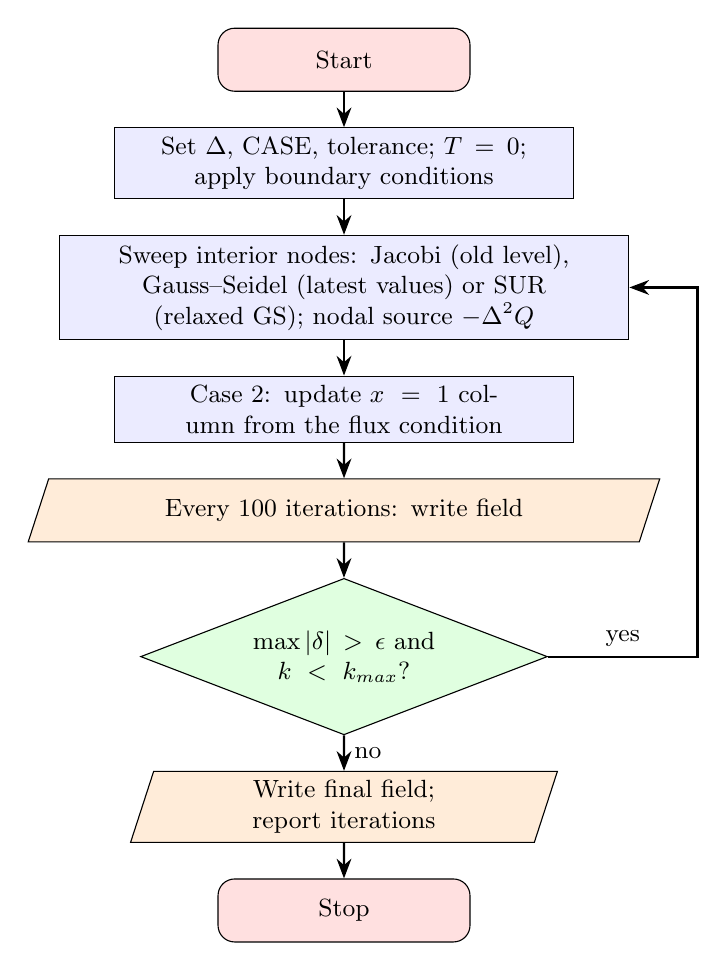
\begin{tikzpicture}[node distance=0.45cm]
\node(s)[startstop]{Start};
\node(i)[process,below=of s]{Set $\Delta$, CASE, tolerance; $T=0$; apply boundary conditions};
\node(sw)[process,below=of i,text width=7.0cm]{Sweep interior nodes: Jacobi (old level), Gauss--Seidel (latest values) or SUR (relaxed GS); nodal source $-\Delta^2Q$};
\node(n)[process,below=of sw]{Case 2: update $x=1$ column from the flux condition};
\node(o)[io,below=of n]{Every 100 iterations: write field};
\node(d)[decision,below=of o]{$\max|\delta|>\epsilon$ and $k<k_{max}$?};
\node(f)[io,below=of d]{Write final field; report iterations};
\node(e)[startstop,below=of f]{Stop};
\draw[arrow](s)--(i);\draw[arrow](i)--(sw);\draw[arrow](sw)--(n);\draw[arrow](n)--(o);\draw[arrow](o)--(d);
\draw[arrow](d)--node[right,font=\small]{no}(f);\draw[arrow](f)--(e);
\draw[arrow](d.east)--node[above,font=\small]{yes}++(1.9,0)|-(sw.east);
\end{tikzpicture}\caption{Common structure of \texttt{code/jacobi.c}, \texttt{gauss\_seidel.c} and \texttt{sur.c}.}\end{figure}

\section{Code review and corrections}
The three codes were taken from the submitted report (\texttt{original/code\_from\_report/}). Run unchanged on the three grids, the Gauss--Seidel and SUR codes reproduce the Case~1 iteration counts of the original table exactly (91/308/4441 and 165/553/7753), and so does Jacobi for $\Delta=0.05$ and 0.01 (559, 7491). For $\Delta=0.1$ the Jacobi code gives 166 iterations, which is the Case~2 entry of the table, so the two Jacobi entries at $\Delta=0.1$ appear to be interchanged. The following defects were corrected:
\begin{table}[H]\centering\small
\begin{tabular}{p{3.6cm}p{7.0cm}p{4.4cm}}\toprule
Location & Problem & Correction\\\midrule
Jacobi, \texttt{setBoundaryConditions} & \texttt{T[MX-1][NY] = T\_min} writes one element beyond the end of \texttt{T} (undefined behaviour) and the right wall is never set. & Index \texttt{[MX-1][j]}.\\
all three, boundary conditions & $T_{max}$ was applied on $y=0,1$ and $T_{min}$ on $x=0,1$, i.e.\ the problem was rotated by $90^\circ$ relative to the statement (Case 1: $T=10$ on $x=0,1$, $T=0$ on $y=0,1$). For a square with these symmetric conditions the field is merely rotated, but it is inconsistent with the stated problem and with the source positions. & Boundary values applied as stated.\\
all three, source location & \texttt{(int)(0.45/delta\_x)} truncates $44.999\ldots$ to 44 for $\Delta=0.01$: the source sat at $x=0.44$, the sink at $0.55$. & Rounding to the nearest node.\\
all three, output & The whole field was written every iteration ($\approx0.7$~GB for $\Delta=0.01$; the 2.6~GB files in the original folders have the same cause). & Written every 100 iterations and at the end.\\
Case 2 & Not present in the submitted listing although Case~2 results are tabulated. & Added with a \texttt{CASE} switch and a second-order flux closure.\\\bottomrule
\end{tabular}\caption{Defects and corrections (marked \texttt{[FIX]}/\texttt{[ADDED]} in \texttt{code/}).}\end{table}
Not changed: the nodal interpretation of $Q$, the iteration formulas, the relaxation factor, the tolerance and the use of \texttt{float} in the Jacobi code (adequate for $\epsilon=10^{-4}$, but it limits the attainable tolerance to $\sim10^{-6}$ for $T\sim10$). The value 12\,345 in the original Case~2 table exceeds the iteration cap (\texttt{Max\_iteration} $=10\,000$) of the listed codes and could not be reproduced.

\section{Results}
\subsection{Temperature fields}
\begin{figure}[H]\centering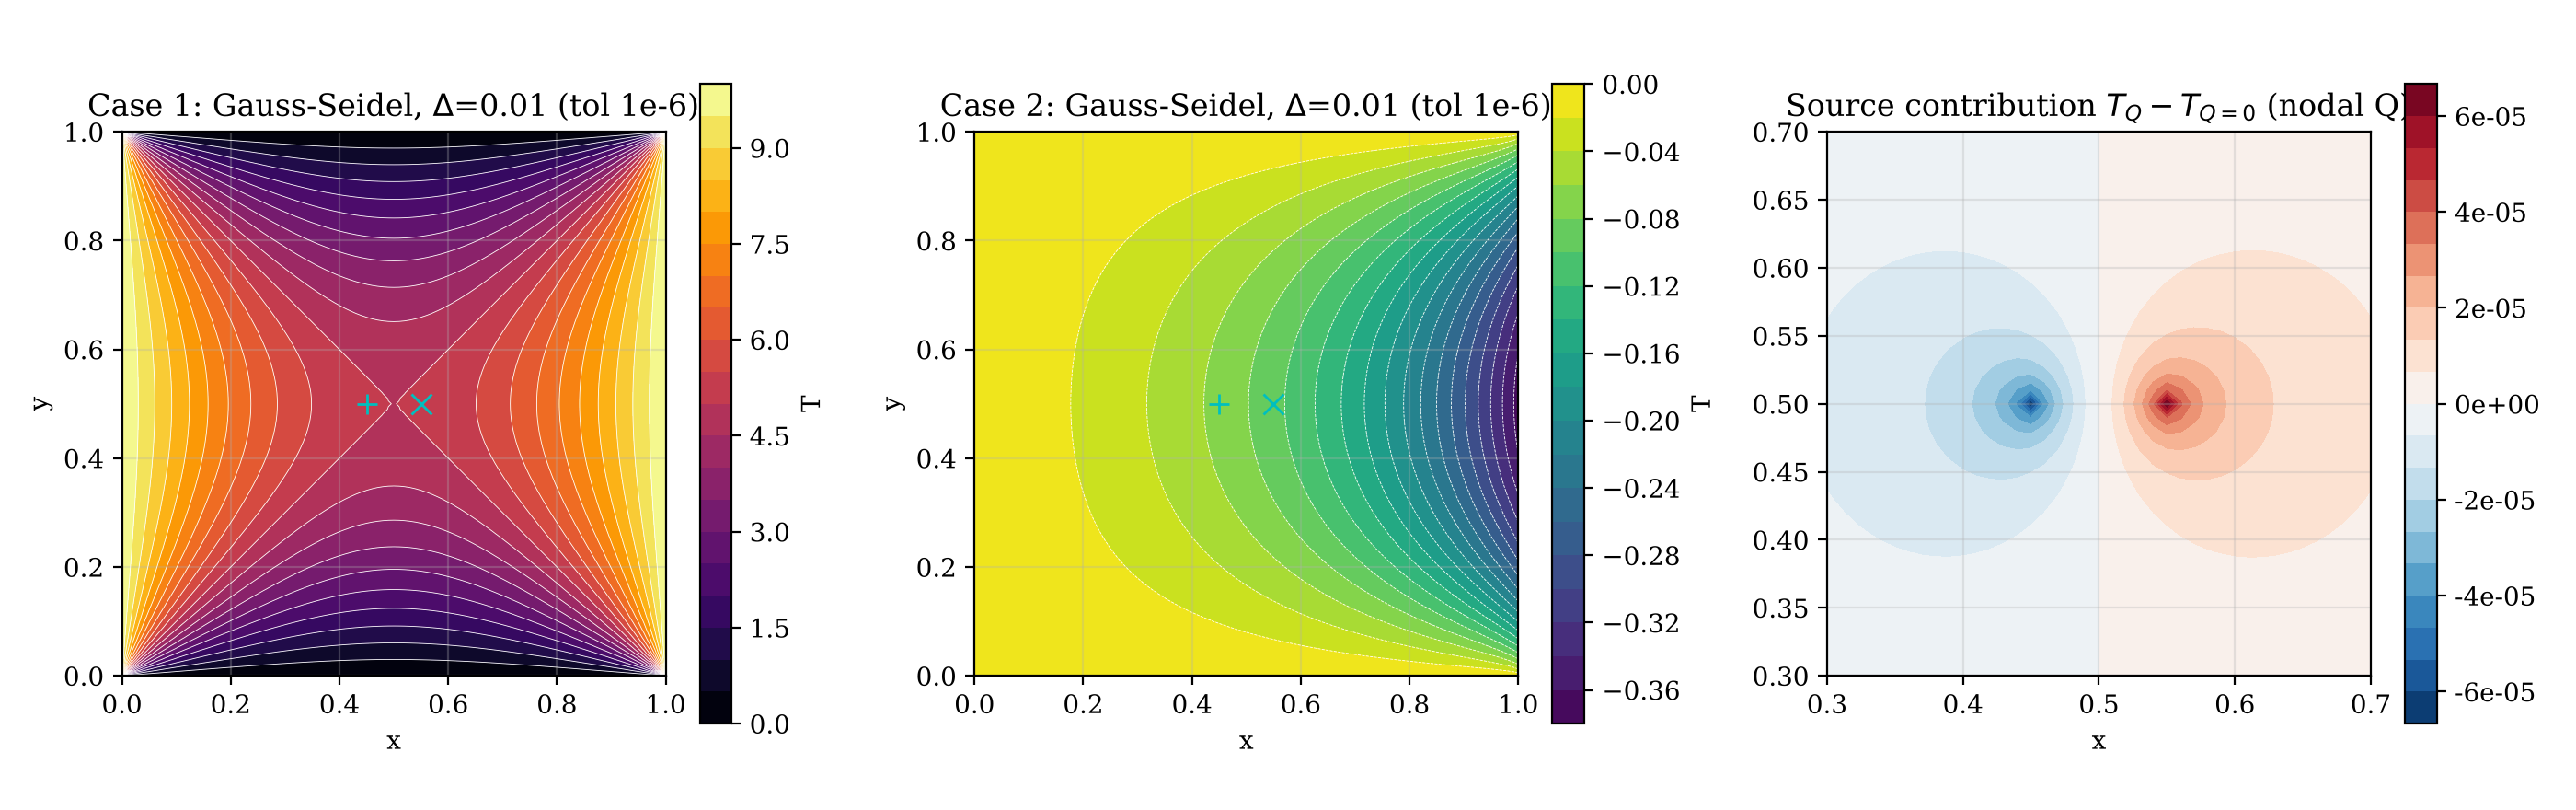
\includegraphics[width=\textwidth]{../results/fig1_contours_and_source_effect.png}
\caption{Converged fields ($\Delta=0.01$, Gauss--Seidel, tolerance $10^{-6}$) for Cases 1 and 2, and the contribution of the nodal sources ($+$: source, $\times$: sink).}\end{figure}
Case~1 is symmetric about both centre lines with a saddle at the centre ($T=5$ exactly, by symmetry). In Case~2 the outward flux through $x=1$ draws the temperature negative; the minimum, $T(1,0.5)=-0.37$, lies at the middle of the flux boundary.

\subsection{Effect of the sources}\label{sec:source}
With $Q$ defined as a nodal value, the source and sink together perturb the field by at most $6.2\times10^{-5}$ (right panel above): the source strength integrated over one cell is $Q\Delta^2$, which vanishes as the grid is refined. If a unit \emph{point} source were intended ($\int Q\,dA=\pm1$), the nodal value must scale as $Q=\pm1/\Delta^2$; this case (not part of the original assignment, shown as an extension in \texttt{results/fig5\_extension\_point\_dipole.png}) produces a dipole of amplitude $0.62$. The problem statement should specify which definition is meant.

\subsection{Accuracy of the discretisation}
\begin{figure}[H]\centering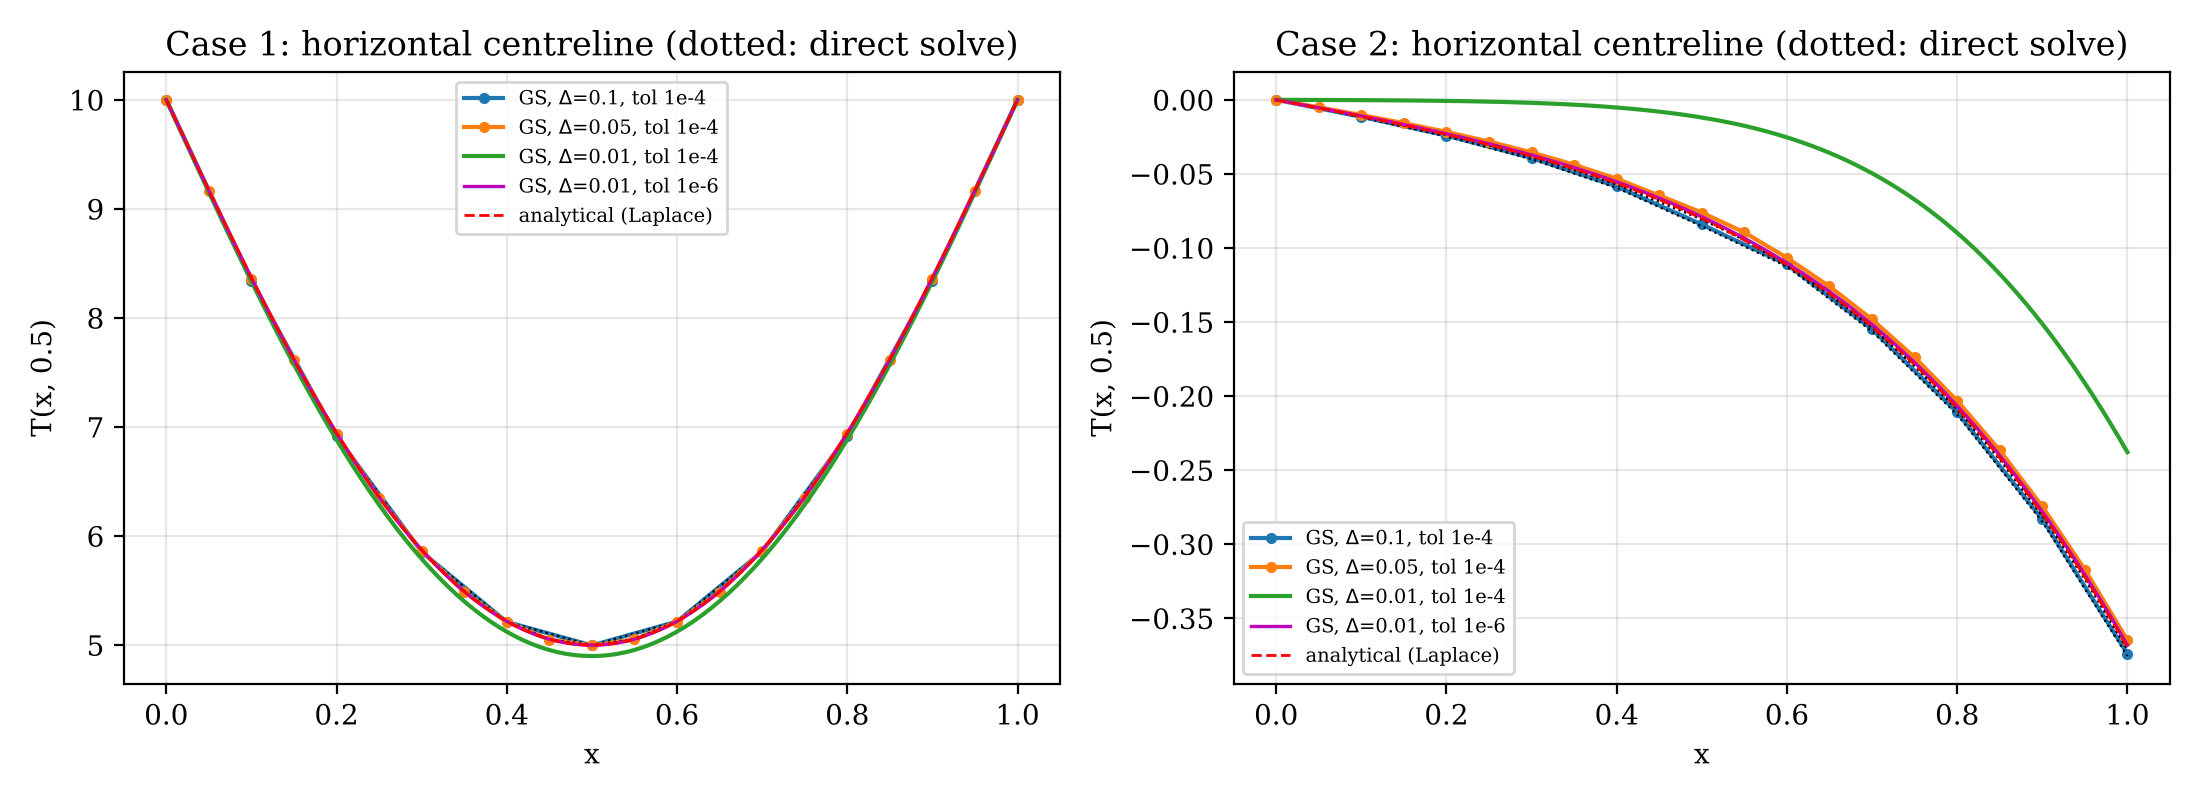
\includegraphics[width=\textwidth]{../results/fig4_centreline.png}
\caption{$T(x,0.5)$: Gauss--Seidel results at both tolerances, direct solution of the discrete system (dotted) and analytical Laplace solution (dashed).}\end{figure}
\begin{table}[H]\centering\small
\begin{tabular}{cccc}\toprule
$\Delta$ & Case 1: $\max|T_h-T|$ on $[0.2,0.8]^2$ & Case 2: same & Case 2: $|T_h-T|$ at centre\\\midrule
0.1 & $2.97\times10^{-2}$ & $5.39\times10^{-3}$ & $5.26\times10^{-3}$\\
0.05 & $7.99\times10^{-3}$ & $1.56\times10^{-3}$ & $7.49\times10^{-4}$\\
0.01 & $3.30\times10^{-4}$ & $9.01\times10^{-5}$ & $3.20\times10^{-5}$\\\bottomrule
\end{tabular}\caption{Discretisation error of the exact discrete solution.}\end{table}
Halving $\Delta$ reduces the Case~1 error by $3.7$ and the five-fold refinement from 0.05 to 0.01 by $24\approx5^2$, confirming second-order accuracy.

\subsection{Convergence and the stopping criterion}\label{sec:conv}
\begin{table}[H]\centering\small
\begin{tabular}{ccc rr rr rr}\toprule
&& & \multicolumn{2}{c}{Jacobi} & \multicolumn{2}{c}{Gauss--Seidel} & \multicolumn{2}{c}{SUR ($\alpha=0.7$)}\\
Case & $\Delta$ & & iter. & error & iter. & error & iter. & error\\\midrule
1 & 0.1 & $\epsilon=10^{-4}$ & 166 & $1.9\times10^{-3}$ & 91 & $9.1\times10^{-4}$ & 165 & $1.3\times10^{-3}$\\
1 & 0.05 & & 559 & $7.9\times10^{-3}$ & 308 & $4.0\times10^{-3}$ & 553 & $5.2\times10^{-3}$\\
1 & 0.01 & & 7\,486 & $0.201$ & 4\,441 & $0.101$ & 7\,753 & $0.132$\\
2 & 0.1 & & 134 & $3.2\times10^{-3}$ & 84 & $1.6\times10^{-3}$ & 143 & $2.1\times10^{-3}$\\
2 & 0.05 & & 360 & $1.3\times10^{-2}$ & 233 & $6.5\times10^{-3}$ & 393 & $8.5\times10^{-3}$\\
2 & 0.01 & & 761 & $0.214$ & 982 & $0.132$ & 1\,343 & $0.161$\\\midrule
1 & 0.01 & $\epsilon=10^{-6}$ & 19\,426 & $5.7\times10^{-4}$ & 9\,106 & $1.0\times10^{-3}$ & 16\,419 & $1.3\times10^{-3}$\\
2 & 0.01 & & 13\,601 & $3.1\times10^{-3}$ & 7\,909 & $1.6\times10^{-3}$ & 13\,854 & $2.1\times10^{-3}$\\\bottomrule
\end{tabular}
\caption{Iterations and remaining iteration error $\max|T^k-T_{direct}|$.}\end{table}
\begin{figure}[H]\centering
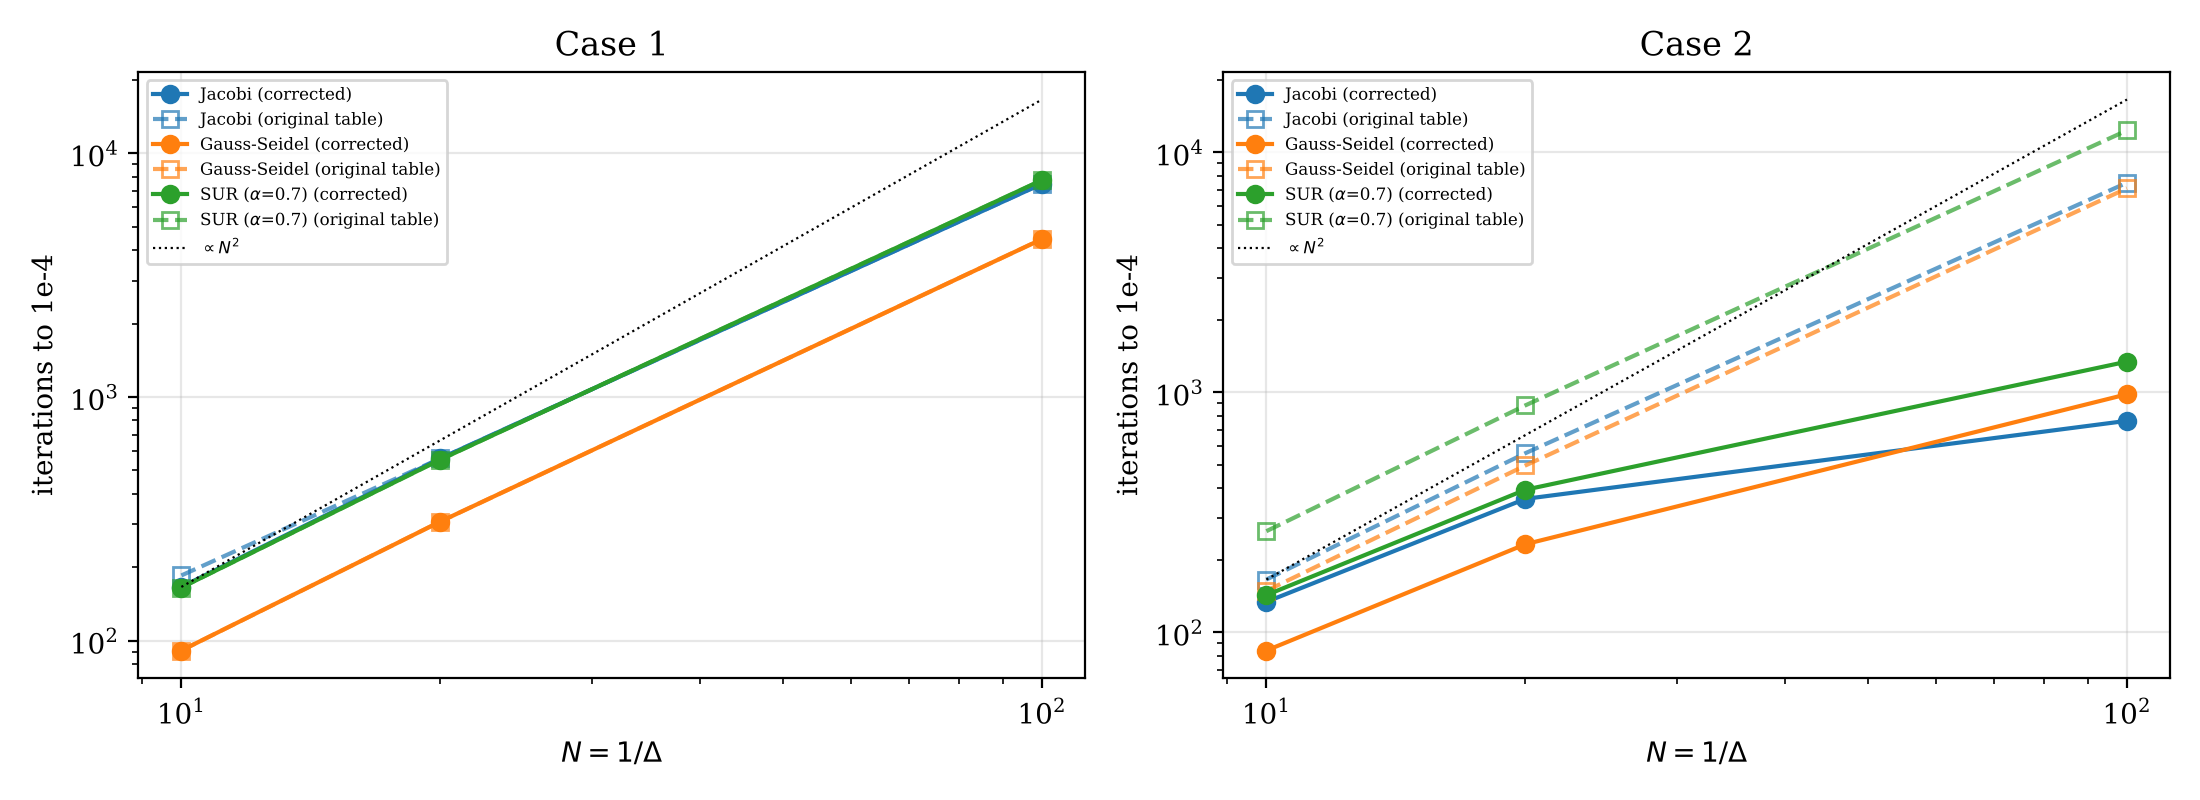
\includegraphics[width=\textwidth]{../results/fig2_iterations_vs_grid.png}
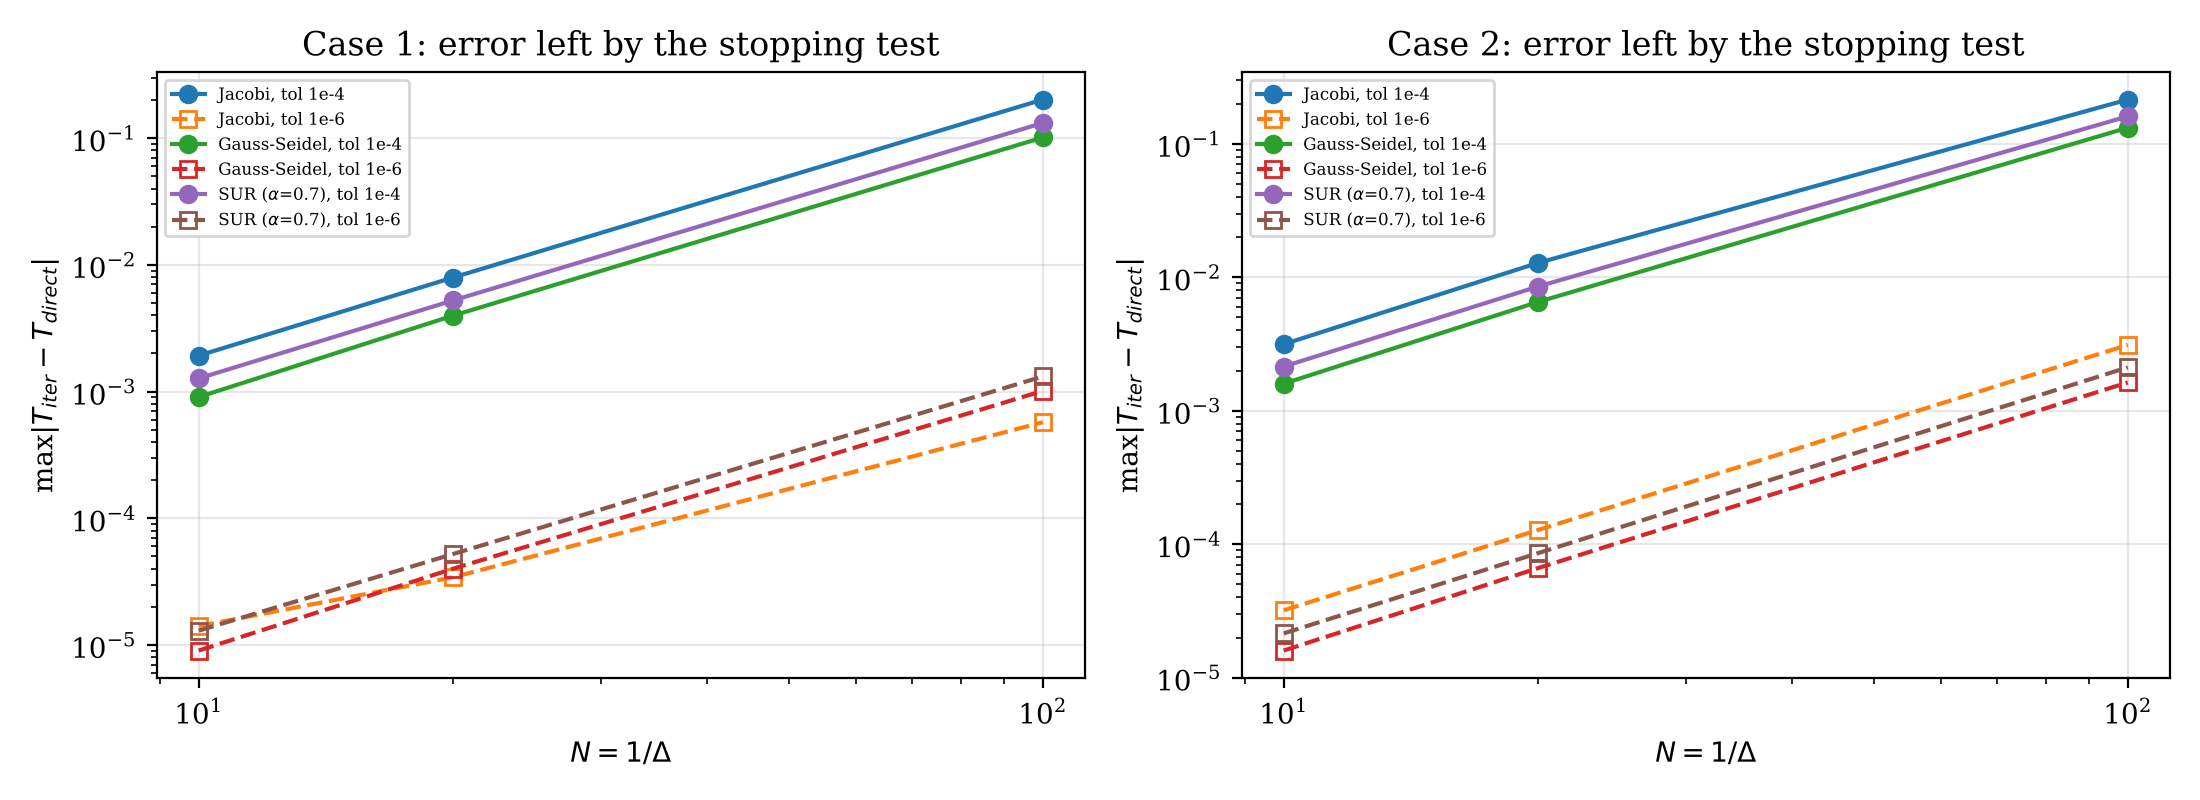
\includegraphics[width=\textwidth]{../results/fig3_termination_error.png}
\caption{Top: iterations to $\epsilon=10^{-4}$ against $N=1/\Delta$ (corrected codes and the original table). Bottom: iteration error remaining at termination for both tolerances.}\end{figure}
\begin{itemize}
\item \textbf{Case 1} follows the theory: Gauss--Seidel needs $\approx0.55$--$0.6$ of the Jacobi iterations, SUR with $\alpha=0.7$ needs about as many as Jacobi, and the counts grow roughly as $N^2$.
\item \textbf{The remaining error matches Eq.~\eqref{eq:err}.} At $\Delta=0.01$, $\epsilon\rho/(1-\rho)=0.20$ (Jacobi) and $0.10$ (Gauss--Seidel), against the measured $0.201$ and $0.101$.
\item \textbf{Case 2 is under-converged at $\epsilon=10^{-4}$.} Its solution is small ($|T|\le0.37$) and grows slowly from the zero initial guess, so the increments fall below $10^{-4}$ long before convergence (761--1\,343 iterations at $\Delta=0.01$), leaving errors of more than half the solution magnitude. With $\epsilon=10^{-6}$ the iteration counts rise to 7\,900--13\,900 and the error falls to $\le3\times10^{-3}$. The original Case~2 counts (7\,081--12\,345) are of this order, which suggests that the original Case~2 code used a different flux closure or tolerance.
\end{itemize}

\section{Conclusions}
\begin{itemize}
\item The corrected solvers converge to the direct solution of the discrete Poisson problem, which is second-order accurate ($3.3\times10^{-4}$ interior error at $\Delta=0.01$ for Case 1).
\item Iteration counts scale as $\Delta^{-2}$; Gauss--Seidel is about twice as fast as Jacobi, and under-relaxation slows convergence for this linear problem.
\item An absolute increment tolerance is not an error estimate: on the $101\times101$ grid $\epsilon=10^{-4}$ leaves errors of $0.1$--$0.2$, and in Case~2 more than 50\% of the solution. A residual-based or relative criterion, $\epsilon\sim(1-\rho)\times$ target accuracy, should be used.
\item As defined (nodal $Q=\pm1$), the source pair changes the solution by less than $10^{-4}$; a unit point dipole would require $Q=\pm1/\Delta^2$.
\end{itemize}

\section*{Reproducing the results}
\texttt{bash run.sh} builds and runs all 18 combinations at $\epsilon=10^{-4}$ and again at $\epsilon=10^{-6}$ (only the constants are substituted), then calls \texttt{code/postprocess.py} (NumPy, SciPy, Matplotlib). Total run time is about 25~s.

\appendix\section{Corrected source: Gauss--Seidel}
\lstinputlisting[language=C]{../code/gauss_seidel.c}
\end{document}
